%===================================== CHAPTER 8 Implementation =================================

\chapter{Implementation}

This chapter discusses the details of the system implementation process, both for front end and back end implementation but also how the project was managed through out the process.


\section{Project Progression}
Project progression is derived from the activity plan \todo{ref{app:activityplan}}, meeting minutes \todo{ref{app:meetingabstract)}} and Trello archive \todo{Blir dette referet til? + legg inn ref her. Står det noe om hvor lange sprintene er tidliger? når de slutter of started klokkeslett}  and will only briefly summarize what was done at each sprint and only serves as a "quick tour" through the development process  

\begin{description}
	
	\item[Sprint 1 - 23.01.15 - 30.01.15] \hfill \\ 
	The first week mainly consisted of getting familiar with each other and the assignment. As soon as the introductions were done, we talked about our personal goals to set the expectation as a group. We formalized the rules of engagement \textbf{Figure \ref{fig:rules_of_engagement}} for the group to sign, and also delegated responsibilities. Later we established a meeting agenda with the customer and met with them for the first time.
	
	\item[Sprint 2 - 30.01.15 - 06.02.15] \hfill \\ 
	In sprint 2 we began planning and formalizing the requirements. Large sections of work like sketching a WBS {Figure \ref{Fig:wbs}}, generating a product backlog \todo{ref til appendix / legg in i appendix?}, and making use cases were done this week. Other design work like the architecture and UI mock-ups were also started on.
	
	\item[Sprint 3 - 06.02.15 - 13.02.15] \hfill \\ 
	This was the first week of development. We started testing the API \textbf{Section \ref{subsec:api}} and finalized some paper prototypes for user testing, \todo{Referanse til papirprototype} and also completed the design for the database and overall system architecture. Research towards the personalization, the front end framework \textbf{Section \ref{subsec:ionic}} \todo{ref:personalization} and differences between the two operating systems \todo{ref crossplatform OS} was also done. 
	
	\item[Sprint 4 - 13.02.15 - 20.02.15] \hfill \\ 
	Analyzing the past work \ref{subsec:stedr} to see if would fit our needs, continuing the research towards collaborative filtering \ref{sec:personalization_algorithms}. Also learning docker \ref{subsec:docker}. Mapping the Digitalt fortalt \todo{ref} categories to our own and conducting and evaluating the paper prototype tests as well. During this sprint the database code was also starting to take shape. Prioritizing the functional requirements done in order to better plan the next sprint.  
	
	\item[Sprint 5 - 20.02.15 - 27.02.15] \hfill \\ 
	In this sprint we manage to get the harvesting up and running after the database was ready. A lot of work with the internal models on the backend was done. The frontend team moved steadily though the initial work on on the prioritized views.(login, story and list.) there was also a revision of the prototype to accommodate costumer and user-test feedback.
		
	\item[Sprint 6 - 27.02.15 - 06.03.15] \hfill \\ 
	Finalizing the database communication was done in order to fully test frontend and to get the backend team to get started on the personalization. The testplan was in stage of being attuned and formalized for the documentation. After the new prototype was finished there was conducted new usertest and the worked continued on each of the application views.
	
	\item[Sprint 7 - 06.03.15 - 13.03.15] \hfill \\ 
	Some work to meet a report delivery was done early in the sprint. ahead in the sprint backend was showing good progress on finding/testing a suitable filtering framework. While fronted refined the look of each view to better fit the users needs. but also working out some issues with the server communication.
	
	\item[Sprint 8 - 13.03.15 - 20.03.15] \hfill \\ 
	The application was taking shape on many fronts so this week we worked more on video support and started on the on-boarding section of the application. On the backend the Mahout\todo{ref til mahout}  framework setup was on the way. There was also used some resources on testing.

	\item[Sprint 9 - 20.03.15 - 27.03.15] \hfill \\ 
	Polishing some features and functionality to hit the milestone (Beta version) this week so the the application was ready for some testing in the wild the upcoming easter. Further development on the Mahout framework, content-based filtering and fixed some unforeseen issues on the harvester was the done on the serverside.
	
	\item[Easter - 27.03.15 - 07.04.15] \hfill \\ 
	The application was tested under informal conditions on family and friends, a so-called "in the wild" test.
	
	\item[Sprint 10 - 08.04.15 - 17.04.15] \hfill \\ 
	We dealt with the feedback from the test conducted during the passover \todo{Blir dette riktig?} . which some of teh problems where platform specific. Did some more polish on the  views and cleared out some frontend bugs. on backend work continued on filtering both collaborative and content-based witch it would for the rest of the sprints. 

	\item[Sprint 11 - 17.04.15 - 24.04.15] \hfill \\ 
	The application is beginning to be close finished on a functional level. Resource dedicated to polish and bugsfixing increased while a lot of testing was conducted on the server. while the last big task on backend was to finalize the filtering.

	\item[Sprint 12 - 24.04.15 - 01.05.15] \hfill \\ 
	Sprint 12 was similar to sprint 11 but there were a lot more hours used this week due to the a next milestone. Final build (costumer ready) which we intended to hit at the end of this week. This did not happen but since we aimed for a final build for 1th of may we had some time for some last minute changes and fix undiscovered bugs which was the case. we also used some extra time for component and system testing and the filtering was done this week.
	
	\item[Sprint 13 - 01.05.15 - 08.05.15] \hfill \\ 
	This week was mainly bug fixing for some member for the group while the majority did a lot og report and documentation work. Planning a acceptance test with the costumer the following week. We walked through the application and did extensive functional tests prior to the costumer meeting 

	\item[Sprint 14 - 08.05.15 - 15.05.15] \hfill \\ 
	During the tests the week before more undiscovered issues was uncovered and we needed some more time for polish and fixing. We had not yet locked in a date for the costumer to do a acceptance test other the before the end of the month so the costumer did not appeal, and agreed to set up a final meeting the following Monday. Which we felt very confident we would take care of our main concerns and give us some time to go the extra mile.
	
	\item[Past 15.05.15] \hfill \\ 
	At the start of the week we meet with the costumer to go go through the functionality in conjunction with the functional requirements to see if the costumer also thought we hit our goal\todo{ref til acceptance test}.
	  
	Work was conducted after the last sprint(sprint 14) this was mainly fixing some bugs, finalizing the report and the application and source code handover.
	
\end{description}

\begin{figure}[h!]
	\centering
	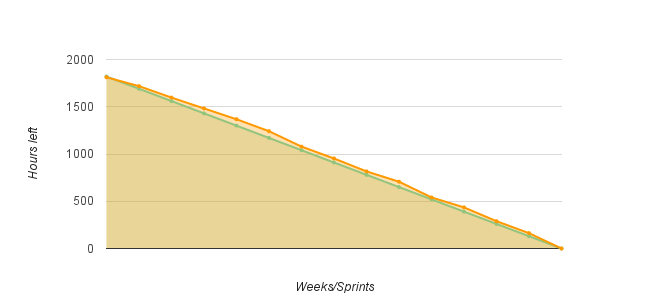
\includegraphics[width=\textwidth]{fig/burnDownAfter}
	\caption{final burn down chart}
	\label{Fig:burnDownAfter}
\end{figure}

\section{Front end}

In this section will be an elaboration of some challenges and limitations during the creation of the user interface, both concerning the design and the implementation aspects of the process.

\subsection{User interface}

Early on in development, the team discovered several limitations of the Ionic framework. For example when using a list to display stories, it was not possible to swipe the list both left and right. The idea was to swipe one way to add a story to be read later, and swipe the other way to reject a story from the list entirely.  Because this proved to be impossible, the views were redesigned into a different solution which was much less based around swiping.\newline

As this is an application for mobile devices, it had to be adapted to work on different screen sizes. The team found that it would most likely be best to target a relatively small screen size and then simply enlarge it for bigger screens. This eliminated the issue of having to compress the components to fit smaller screen sizes and potentially be forced to redesign the whole view to fit small screens.\newline

The target audience for the application included both those who have an interest in cultural activities, and also those who do not have any interest or experience about this, so as to encourage more of the general population to discover an interest in the subject. A specific target audience of 16-19 year old teenagers were promoted as a possible focus, because of the possibility of encouraging a young audience to develop an interest in cultural heritage. However, this was not stated until around  midway in the project timeline. This fact made it difficult to consider target audience when making design decisions. \newline

The applications uses many different icons in various parts of the interface, and these have been the source of much debate and redesign. The icons used to represent categories were not always understood by users, and some categories like “local tradition and food” were difficult to represent universally with just a single icon. Also the bookmark icon shown in the upper right area of figure 8.xx was confusing to many users, and there was a concern in the team that this icon might not accurately represent that it allows the user to save the story in a collection.\newline

Adopting accurate naming conventions for the different components has also been a considerable issue. Stories can be saved in collections, but these collections have interchangeably been called lists, tags, and bookmarks in the system. Also when asking a user to input their preferred categories to receive stories from, there has been some confusion because of interchangeably calling these categories for interests,  preferences, and categories.\newline

Implementing media, and especially video, has been a challenge in the project. An issue with this has been that playing videos is handled differently on iOS and Android, which had resulted in some bugs that only appear on one platform and not the other. These types of issues have been problematic to fix and has taken up much time. In addition, the videos provided by the Digitalt fortalt website come from different sources. Some of them are Youtube videos, others are Vimeo videos, and there are also other variations. Integrating all these different formats smoothly into the application has been a considerable challenge as well.

\subsection{Prototype}

The prototype has been through multiple iterations. Early on, it was imagined to have a sort of “magic” discovery function where a user would for example rub a crystal ball and receive a recommended story. This idea was later discarded because the team and customer realized
 it would be better usability to present the user with multiple recommended stories that they could simply browse through instead.\newline

Another of the early ideas was for the user to receive a “daily story” or some sort of schedule for being presented with recommended stories. However, due to workload and time constraints, this requirement was heavily down-prioritized. The most important parts were the personalization and usability aspects, so receiving notifications seemed like an unnecessary extra feature.\newline

A big issue for the interface design has been the handling of the different media elements (text, pictures, audio, video) and how these should be positioned relative to each other. For a while the team designed the application to have one tab for each of these four elements in the story view, as shown to the left in \textbf{Figure \ref{Fig:prototype}}. The customer had a concern that this might not be the optimal solution, as a user would for example not be able to read text and view pictures simultaneously. After some discussion, the interface was redesigned so that the text would be persistent, and instead the user could tab between pictures, audio, and video. The resulting design can be seen to the right in \textbf{Figure \ref{Fig:prototype}}. 

\begin{figure}
	\centering
	\begin{subfigure}[h]{0.4\textwidth}
		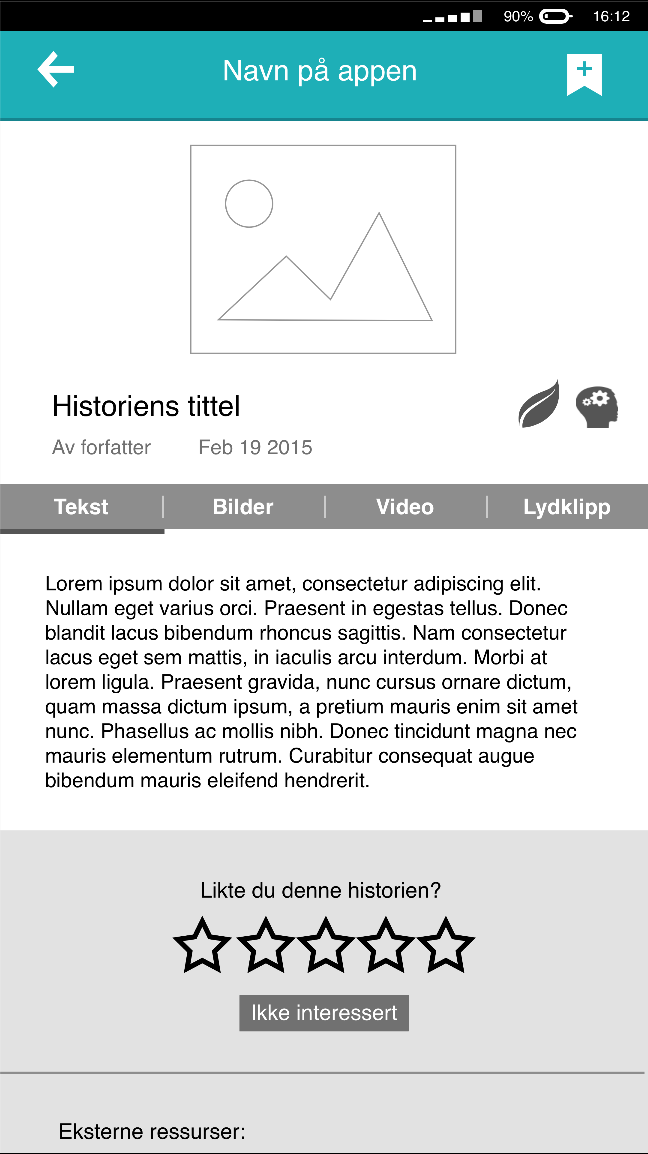
\includegraphics[width=\textwidth]{fig/prototype1}
	\end{subfigure}
	\begin{subfigure}[h]{0.4\textwidth}
		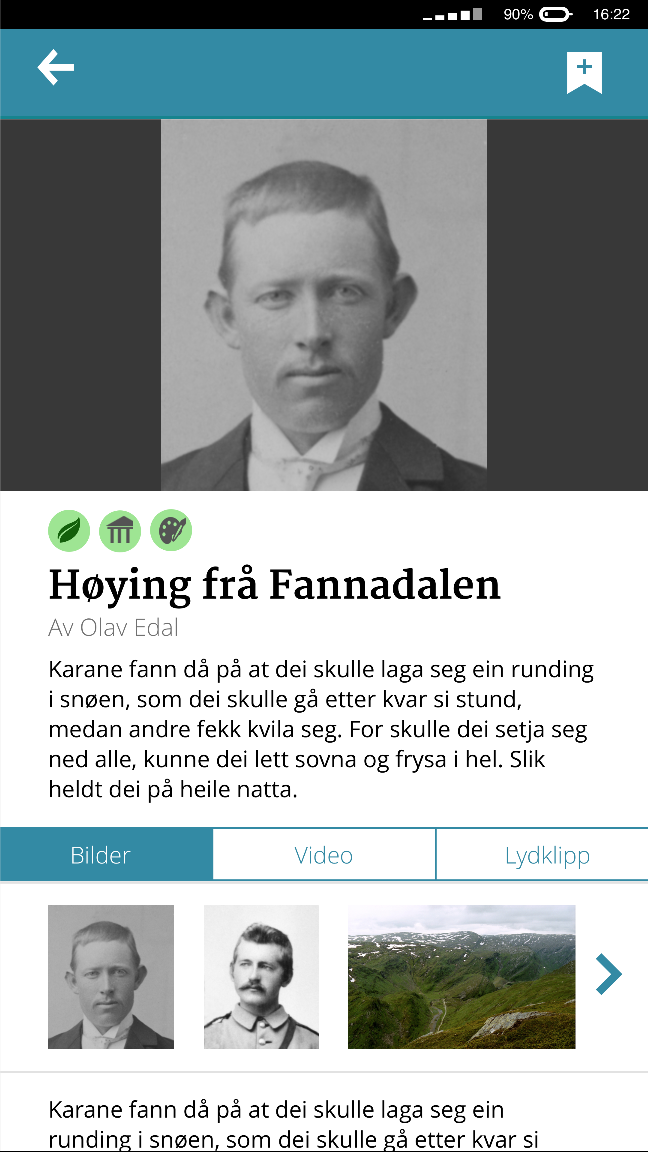
\includegraphics[width=\textwidth]{fig/prototype2}
	\end{subfigure}
	\caption{Comparison of the story view in the first and second versions of the prototype.}
	\label{Fig:prototype}
\end{figure}

\section{Back end}

This section describes the development of each part of the back end. It aims to give a timeline of the development and explain how and why important decisions were made. The different parts described here are the database and the personalization.  

\subsection{Database}

Based on the first version of the functional requirements for the application, an initial ER-diagram was made in the middle of February. At this stage the customer and the team had not come to an agreement on a prioritization of the non-functional requirements. This meant that it was for instance not clear how important the performance of the system would be for the customer, an attribute of the system which would influence how much info should be stored for each story in the database versus how much info should be retrieved from Digitalt fortalt every time a user views a story. However, the changes to the initial diagram have been relatively minor. Some of the alterations were based on updated requirements from the customer, while others stemmed from the group and were optimization of the data model or changes made to facilitate the personalization. \newline

Shortly after the first ER-diagram was made, an SQL script for creating a database was also made. Since the ER-diagram has undergone changes for quite some time after the first version was made, these changes have also influenced the SQL script. This means that a change in the data model has lead to more work than just updating the ER-diagram. However, the progress of the project relied on testing against an operational database, for instance regarding the harvesting of stories from Digitalt fortalt. \newline

The relational database was mapped from the ER-diagram using the algorithm in \cite[p.270-278]{AS2}. Some of the tables in the database has the potential for NULL values, but this was accepted as it was considered more important to keep the mapping from a entity to a table. In addition, the database already had quite a few tables and further splitting would make the extraction of information more costly, with numerous join operations. \newline 

The customer had early on said that the retrieval of research data about the use of the application was important for them. Initially, the details of this was not properly formulated and the initial data model therefore did not reflect this. After receiving a detailed list from the customer describing the research data to be gathered, alterations - mostly additions - in the data model were made to accommodate this. This concerned storing timestamps for user actions and states of stories.  \newline

The team did not decide or understand how to do the personalization until mid March. This decision introduced changes to existing tables and the need to create additional tables and views in the database. Mahout had requirements for the input data, which meant that a view was created to store all the necessary data for collaborative filtering. Using this view made it straightforward to put the desired data from the database into Mahouts data model.

\subsection{Personalization}

At the start of the project much time was devoted to understanding content-based and collaborative filtering and how the theoretical descriptions of these techniques could be turned into a practical implementation in our application. When the back end part of the group had a better understanding on how this could be done, an important decision was whether to use open source recommender engines or to implement the algorithms ourselves. After studying the math and complexity involved in writing our own implementation it became clear that the best solution would be to use existing recommender engines, even if this would require some adjustments to already written code. \newline

As the project was nearly halfway through when the decision to use an open source recommender engine was made, the team did not find the time to do a thorough review of the many different alternatives. This increased the probability of choosing the wrong tool to work with and violated the stated preventive action in the risk list (see \textbf{Appendix \ref{app:risklist}}). However, the customer suggested three different recommender engines that might be worth looking into, one of which was Mahout. In choosing a tool the customer had done some research on, the group found that the risk of making a wrong choice decreased somewhat. In addition, Mahout presented its features in a way that resembled the groups research on filtering algorithms and it was therefore reason to believe that getting started with Mahout would not require much additional research. Of particular importance was the fact that Mahout offered an explanation on how to do content-based filtering using their recommender engine. Most such engines provided functionality for doing collaborative filtering, but it was not always clear how content-based filtering could be done.\newline

Mahouts website provided some guiding on how to build a recommender which made it possible to use the tool without thorough knowledge of how the different methods worked. Most of the work in the beginning of doing the personalization thus centered around how to gather and produce data in a format acceptable to Mahout and how to treat the output recommendations. Content-based filtering was implemented first, as this was the customer's wish and because the first recommendations presented to a user would always be content-based. Since Mahout does not provide methods for finding similarities between items based on their attributes, the group had to implement this. There exist a vast number of functions to compute similarity between objects. The group did some research on different similarity measures, but the literature did not provide a clear-cut answer to which measure was best fitted to our data. Cosine similarity was chosen for its simplicity and because a story's subcategories lent itself well to be represented as a vector.\newline

The customer requested the use of both item-based and user-based collaborative filtering. There was some doubt in the group as to whether the produced recommendations from the two methods could be combined, but it was found that this was possible as both take the same data model as input. When doing user-based collaborative filtering, a threshold value had to be set to tell the recommender engine which users should affect the recommendations. This concerns the similarity found between users. It was difficult to set this value as the computation of the similarity is done by Mahout and because the group did not know what threshold value would be reasonable to set. The value is set by means of trial and error, looking at the resulting recommendations produced using different values, and by looking at example use of this method. \newline

\subsection{Language}
\label{subsec:backend_language}
\textbf{PHP}\newline
PHP is a server-side scripting language that is especially suited for web development produced by The PHP Group \cite{HM8}. It is a general-purpose scripting language often used to provide dynamic content from a web server to a client. During the pre-study period several reasons for choosing PHP as the main back end language were presented. Firstly, all back end team members were experienced in the use of PHP. Secondly, as inexperienced users of Docker, more documentation existed on how to implement PHP with Docker than with the other language alternatives \todo{DO WE HAVE TO WRITE THE LANGUAGE ALTERNATIVES IF I WRITE THIS?}considered.  Lastly, it was easily combined with the HTTP protocol used by front end to request and receive data (see \textbf{Section \ref{subsec:frontend-backend_communication}}).\newline

\noindent\textbf{Java}\newline
Java is a very popular general-purpose object oriented programming language developed by Sun Microsystems and later Oracle Corporation \cite{HM9}. Java was later in the project chosen as a secondary back end language. This was because Mahout, which was used to implement the recommender engine (see \textbf{Section \ref{sec:personalization_how}}), is written in Java. 

\cleardoublepage